\section{Prediction Aggregation}

\begin{table}[p]
  \centering

  \textbf{Results from Experiment 1}

  \vspace{3em}

  \begin{tabular*}{\textwidth}{ l p{3cm} p{1.5cm} p{1.5cm} p{1.5cm} p{1.5cm} p{1.5cm} }
    \toprule
      ~ & \emph{method} & 
      $d_1$ & $d_2$ & $d_3$ & $d_4$ & $d_5$ \\ 
    \midrule
    S & svd1          & 1.2389	  & 1.1260	  & 1.1327	  & 1.1045	  & 1.1184	 \\
    S & svd2          & 1.2630	  & 1.1416    & 1.1260	  & 1.1458	  & 1.1260	 \\
    S & svd3          & 1.0061	  & 0.9825	  & 0.9830	  & 0.9815	  & 0.9797	 \\
    S & svd4          & 1.0040	  & 0.9830	  & 0.9849	  & 0.9850	  & 0.9798	 \\
    S & slope\_one    & 1.1919	  & 1.0540	  & 1.0476	  & 1.0454	  & 1.0393   \\
    S & item\_avg     & 1.0713	  & 0.9692	  & 0.9662	  & 0.9683	  & 0.9725	 \\
    S & baseline       & 1.0698	  & 0.9557	  & 0.9527	  & 0.9415	  & 0.9492	 \\
    S & cosine   	    & 1.1101	  & 0.9463	  & 0.9412	  & 0.9413	  & 0.9382	 \\
    S & pcc       	  & 1.4850	  & 1.1435	  & 1.1872    & 1.2156	  & 1.2022	 \\
    \midrule                                                                    
    A & median    	  & 0.9869	  & 0.8886	  & 0.8857    & 0.8857	  & 0.8855	 \\
    A & average    	  & 0.9900	  & 0.8536	  & 0.8525	  & 0.8525	  & 0.8519	 \\
    A & adaptive       & \textbf{0.9324}	  & \textbf{0.8015}	  & \textbf{0.7993}  & \textbf{0.8238} & \textbf{0.8192} \\
    \bottomrule
  \end{tabular*}

  \vspace{3em}

  \begin{tabular*}{\textwidth}{ l p{3cm} p{2cm} p{2cm} p{2cm} p{2cm} }
    \toprule
      ~ & \emph{method} & 
      \emph{min} & \emph{max} & \emph{mean} & $\sigma$\\
    \midrule
    S & svd1          & 1.1045	& 1.2389	& 1.1441	& 0.2197 \\
    S & svd2          & 1.1260	& 1.2630	& 1.1605	& 0.2277 \\
    S & svd3          & 0.9797	& 1.0061	& 0.9865	& 0.0991 \\
    S & svd4          & 0.9798	& 1.0040	& 0.9873	& \textbf{0.0924} \\
    S & slope\_one    & 1.0393	& 1.1919	& 1.0756	& 0.2415 \\
    S & item\_avg     & 0.9662	& 1.0713	& 0.9895	& 0.2023 \\
    S & baseline       & 0.9415	& 1.0698	& 0.9738	& 0.2196 \\
    S & cosine   	    & 0.9382	& 1.1101	& 0.9754	& 0.2595 \\
    S & pcc       	  & 1.1435	& 1.4850	& 1.2467	& 0.3487 \\
    \midrule            
    A & median    	  & 0.8855	& 0.9865	& 0.9065	& 0.2005 \\
    A & average    	  & 0.8519	& 0.9900	& 0.8801	& 0.2344 \\
    A & adaptive       & \textbf{0.7993}	& \textbf{0.9324}	& \textbf{0.8352}	& 0.2225 \\
    \bottomrule
  \end{tabular*}
  \vspace{2em}

  \caption[Results from Experiment 1]{
    Results from experiment 1 (MovieLens):
    Each cell gives an RMSE value, on the scale 1-5.
    The first table gives errors for each subset of the data ($d_x$).
    Lower values indicate better results.
    Bold values indicate the best result in each column.
    S refers to singular methods, and A to aggregation methods.
    $\sigma$ refers to the standard deviation of each method across the subsets.
  }
  \label{table:results:e1}
\end{table}



done: 4,5

  Results
  ----------------------------------------------------------------------------------------------------
  svd1         	  4: 1.08168	  5: 1.09346	min: 1.08168	max: 1.09346	avg: 1.08757	stddev: 0.076746
  svd3         	  4: 0.9479	    5: 0.94826	min: 0.9479	  max: 0.94826	avg: 0.94808	stddev: 0.013416
  svd4         	  4: 0.94892	  5: 0.9459	  min: 0.9459	  max: 0.94892	avg: 0.94741	stddev: 0.038859
  knn3         	  4: 1.02418	  5: 1.0243	  min: 1.02418	max: 1.0243	  avg: 1.02424	stddev: 0.007746
  knn4         	  4: 1.02304	  5: 1.0244	  min: 1.02304	max: 1.0244	  avg: 1.02372	stddev: 0.026077
  slope_one    	  4: 1.11074	  5: 1.11703	min: 1.11074	max: 1.11703	avg: 1.113885	stddev: 0.05608
  baseline     	  4: 1.10294	  5: 1.10662	min: 1.10294	max: 1.10662	avg: 1.10478	stddev: 0.042895
  cosine       	  4: 1.08539	  5: 1.07813	min: 1.07813	max: 1.08539	avg: 1.08176	stddev: 0.060249
  m_average    	  4: 0.91857	  5: 0.91733	min: 0.91733	max: 0.91857	avg: 0.91795	stddev: 0.0249
  m_median     	  4: 0.92481	  5: 0.9225	  min: 0.9225	  max: 0.92481	avg: 0.923655	stddev: 0.033985
  svd2         	  4: 1.08591	  5: 1.08837	min: 1.08591	max: 1.08837	avg: 1.08714	stddev: 0.035071
  knn1         	  4: 1.18459	  5: 1.1921	  min: 1.18459	max: 1.1921	  avg: 1.188345	stddev: 0.061278
  knn2         	  4: 1.16415	  5: 1.18468	min: 1.16415	max: 1.18468	avg: 1.174415	stddev: 0.101316
  m_svd        	  4: 0.96698	  5: 0.79647	min: 0.79647	max: 0.96698	avg: 0.881725	stddev: 0.291985

  avgs:
  [[:m_svd, 0.881725],
   [:m_average, 0.91795],
   [:m_median, 0.923655],
   [:svd4, 0.94741],
   [:svd3, 0.94808],
   [:knn4, 1.02372],
   [:knn3, 1.02424],
   [:cosine, 1.08176],
   [:svd2, 1.08714],
   [:svd1, 1.08757],
   [:baseline, 1.10478],
   [:slope_one, 1.113885],
   [:knn2, 1.174415],
   [:knn1, 1.188345]]



done 1:

  Results
  ----------------------------------------------------------------------------------------------------
  svd1           	  1: 1.08626	min: 1.08626	max: 1.08626	avg: 1.08626	stddev: 0.0
  svd2           	  1: 1.08119	min: 1.08119	max: 1.08119	avg: 1.08119	stddev: 0.0
  svd3           	  1: 0.94702	min: 0.94702	max: 0.94702	avg: 0.94702	stddev: 0.0
  svd4           	  1: 0.95061	min: 0.95061	max: 0.95061	avg: 0.95061	stddev: 0.0
  knn3           	  1: 1.02663	min: 1.02663	max: 1.02663	avg: 1.02663	stddev: 0.0
  knn4           	  1: 1.02323	min: 1.02323	max: 1.02323	avg: 1.02323	stddev: 0.0
  slope_one      	  1: 1.11015	min: 1.11015	max: 1.11015	avg: 1.11015	stddev: 0.0
  cosine         	  1: 1.07766	min: 1.07766	max: 1.07766	avg: 1.07766	stddev: 0.0
  m_average      	  1: 0.91888	min: 0.91888	max: 0.91888	avg: 0.91888	stddev: 0.0
  m_median       	  1: 0.92529	min: 0.92529	max: 0.92529	avg: 0.92529	stddev: 0.0
  knn2           	  1: 1.1896	min: 1.1896	max: 1.1896	avg: 1.1896	stddev: 0.0
  baseline       	  1: 1.09193	min: 1.09193	max: 1.09193	avg: 1.09193	stddev: 0.0
  knn1           	  1: 1.1808	min: 1.1808	max: 1.1808	avg: 1.1808	stddev: 0.0
  m_svd          	  1: 0.93866	min: 0.93866	max: 0.93866	avg: 0.93866	stddev: 0.0

  avgs:
  [[:m_average, 0.91888],
   [:m_median, 0.92529],
   [:m_svd, 0.93866],
   [:svd3, 0.94702],
   [:svd4, 0.95061],
   [:knn4, 1.02323],
   [:knn3, 1.02663],
   [:cosine, 1.07766],
   [:svd2, 1.08119],
   [:svd1, 1.08626],
   [:baseline, 1.09193],
   [:slope_one, 1.11015],
   [:knn1, 1.1808],
   [:knn2, 1.1896]]



Our first hypothesis, H1, states that:
{
  \itshape
  the accuracy of relevance predictions can be improved
  through adaptive recommender aggregation.
}
The second hypothesis, H2, states:
{
  \itshape
  adaptive aggregation can achieve higher accuracy than global and generalized aggregation methods.
}

In order to verify these hypotheses, we performed adaptive prediction aggregation
through stacked recommenders on the five datasets described in the previous section.
Table \ref{table:results:e1} gives the results from this experiment.
Each cell corresponds to the RMSE values for each dataset,
for each recommender and aggregation approach.
The bottom entry in this table refers to our stacked recommenders method.
As seen in this table, the stacked recommender achieved
lower RMSE values than any of the other applied methods.

Statistics from the results in Table \ref{table:results:e1} 
are given in Table \ref{table:results:e1:sum}.
These values are the minimum, maximum and mean values
for each of the methods. We also include
the standard deviation ($\sigma$) for each method,
across our datasets.
This table confirms the results from the full results table:
Our stacked recommenders approach improves the mean performance
of our system.
The mean performance, along with the standard deviation
are shown in Figure \ref{plot:rmse}.

%\begin{figure*}[!t]
\center

\pgfplotsset{width=\textwidth,height=8cm}
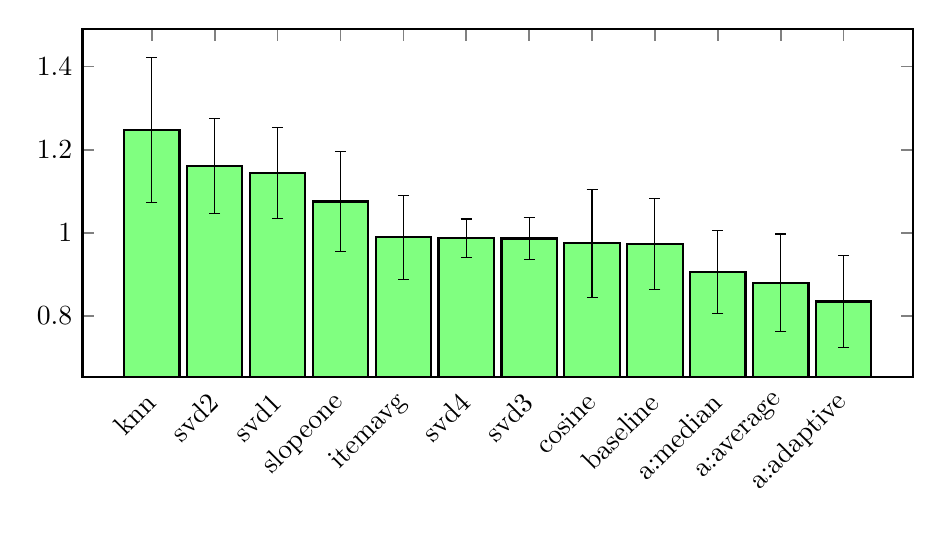
\begin{tikzpicture}

\begin{axis}[
      symbolic x coords={
        knn,svd2,svd1,slopeone,itemavg,svd4,svd3,cosine,baseline,a:median,a:average,a:adaptive},
      xtick=data,
      x tick label style={rotate=45,anchor=east,yshift=-0.5em,xshift=-0.2em},
      bar width=20pt
    ]

    \addplot [ybar,fill=green!50,error bars/.cd,y dir=both,y explicit] coordinates {
      (knn, 1.2467) +- (0,0.17435) 
      (svd2, 1.1605) +- (0,0.11385)
      (svd1, 1.1441) +- (0,0.10985)
      (slopeone, 1.0756) +- (0,0.12075)
      (itemavg, 0.9895) +- (0,0.10115)
      (svd4, 0.9873) +- (0,0.0462)
      (svd3, 0.9865) +- (0,0.04955)
      (cosine, 0.9754) +- (0,0.12975)
      (baseline, 0.9738) +- (0,0.1098)
    %};
    %\addplot [ybar,fill=blue!50] coordinates {
      (a:median, 0.9065) +- (0,0.10025)
      (a:average, 0.8801) +- (0,0.1172)
      (a:adaptive, 0.8352) +- (0,0.11125)
    };
\end{axis}

\end{tikzpicture}
\vspace{-1em}
\caption[Average RMSE Plot]{
  Average RMSE plot: This plot shows the average RMSE for each method, and each aggregation method (denoted "a:").
  The actual numbers are given in Table \ref{table:results:e1}.
  The error bars indicate the standard deviation of each method.
  Note the scale on the y-axis --- the errors are not as pronounced as they might seem. 
}
\label{plot:movielens}
\end{figure*}




\begin{figure}[p]
  \centering
  \subfloat[Experiment 1]{\label{fig:rmse:e1}
\pgfplotsset{width=\textwidth,height=8cm}
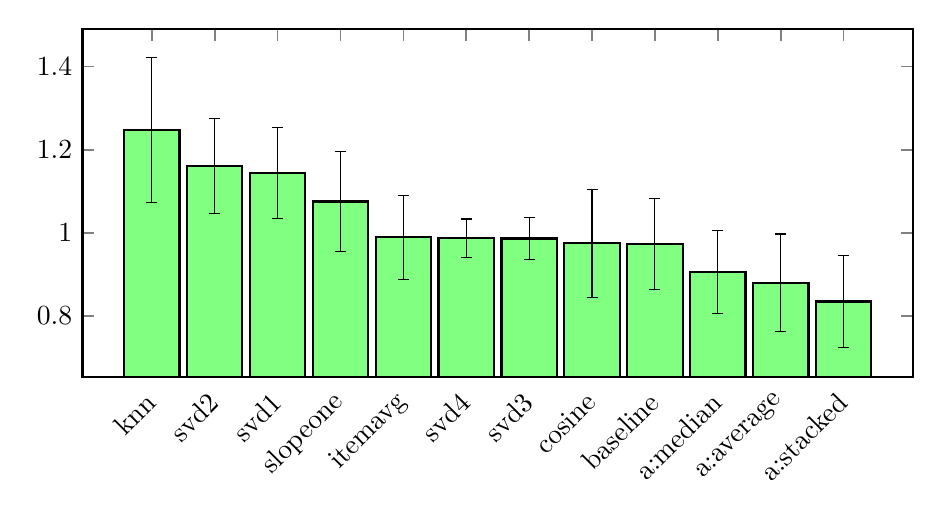
\begin{tikzpicture}
\begin{axis}[
      symbolic x coords={
        knn,svd2,svd1,slopeone,itemavg,svd4,svd3,cosine,baseline,a:median,a:average,a:stacked},
      xtick=data,
      x tick label style={rotate=45,anchor=east,yshift=-0.5em,xshift=-0.2em},
      bar width=20pt
    ]
    \addplot [ybar,fill=green!50,error bars/.cd,y dir=both,y explicit] coordinates {
      (knn, 1.2467) +- (0,0.17435) 
      (svd2, 1.1605) +- (0,0.11385)
      (svd1, 1.1441) +- (0,0.10985)
      (slopeone, 1.0756) +- (0,0.12075)
      (itemavg, 0.9895) +- (0,0.10115)
      (svd4, 0.9873) +- (0,0.0462)
      (svd3, 0.9865) +- (0,0.04955)
      (cosine, 0.9754) +- (0,0.12975)
      (baseline, 0.9738) +- (0,0.1098)
    %};
    %\addplot [ybar,fill=blue!50] coordinates {
      (a:median, 0.9065) +- (0,0.10025)
      (a:average, 0.8801) +- (0,0.1172)
      (a:stacked, 0.8352) +- (0,0.11125)
    };
\end{axis}
\end{tikzpicture}}

\vspace{1em}
 
  \subfloat[Experiment 2]{\label{fig:rmse:e2}
\pgfplotsset{width=\textwidth,height=8cm}
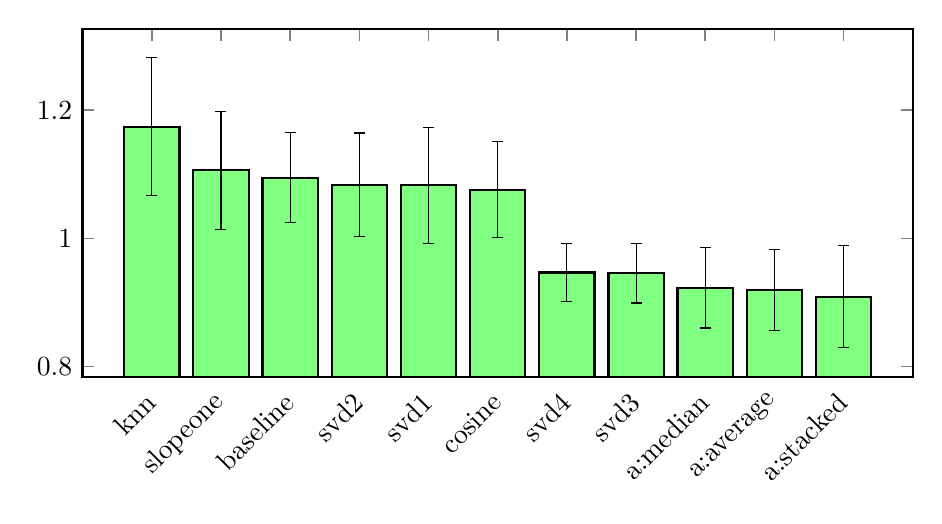
\begin{tikzpicture}
\begin{axis}[
      symbolic x coords={
        knn,slopeone,baseline,svd2,svd1,cosine,svd4,svd3,a:median,a:average,a:stacked},
      xtick=data,
      x tick label style={rotate=45,anchor=east,yshift=-0.5em,xshift=-0.2em},
      bar width=20pt
    ]
    \addplot [ybar,fill=green!50,error bars/.cd,y dir=both,y explicit] coordinates {
      (knn, 1.1740) +- (0,0.1077) 
      (slopeone, 1.1062) +- (0,0.0918)
      (baseline, 1.0945) +- (0,0.0700)
      (svd2, 1.0835) +- (0,0.0808)
      (svd1, 1.0829) +- (0,0.0905)
      (cosine, 1.0760) +- (0,0.0749)
      (svd4, 0.9467) +- (0,0.0446)
      (svd3, 0.9455) +- (0,0.0464)
    %};
    %\addplot [ybar,fill=blue!50] coordinates {
      (a:median, 0.9227) +- (0,0.0626)
      (a:average, 0.9193) +- (0,0.0630)
      (a:stacked, 0.9091) +- (0,0.0797)
    };
\end{axis}
\end{tikzpicture}}

\vspace{1em}

  \caption[Plots of Results for Experiments 1 \emph{\&} 2]{
    Plots of the average RMSEs for Experiments 1 \emph{\&} 2.
    The actual numbers are given in Tables \ref{table:results:e1}
    \emph{\&} \ref{table:results:e2}.
  }
  \label{plot:rmse}
\end{figure}




\begin{figure}
\center
\tiny

\pgfplotsset{width=\textwidth,height=6cm}
\pgfplotsset{every axis/.append style={
thick,
tick style={semithick}}}

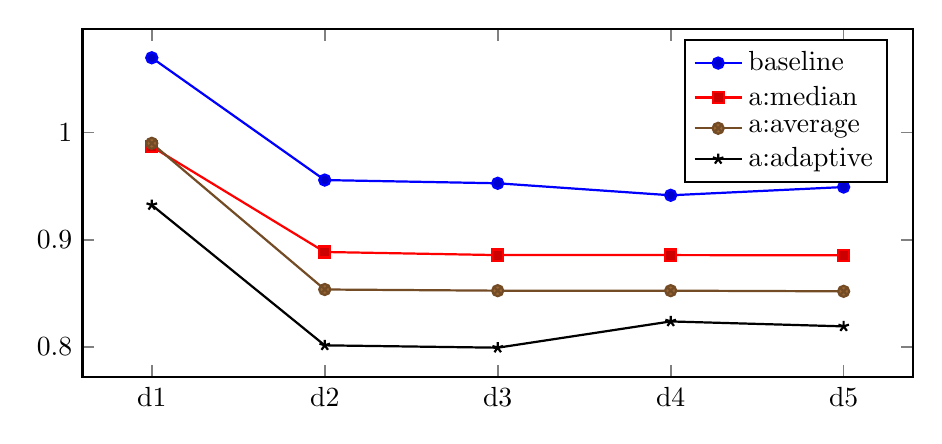
\begin{tikzpicture}

\begin{axis}[
  stack plots=false,
  enlarge x limits=true,
  symbolic x coords={d1,d2,d3,d4,d5},
  xtick=data,
  legend style={
    cells={anchor=west},
    legend pos=north east,
  }
]

\addplot coordinates {
(d1, 1.0698)
(d2, 0.9557)
(d3, 0.9527)
(d4, 0.9415)
(d5, 0.9492)
};
\addlegendentry{baseline}


\addplot coordinates {
(d1, 0.9869)
(d2, 0.8886)
(d3, 0.8857)
(d4, 0.8857)
(d5, 0.8855)
};
\addlegendentry{a:median}
 
\addplot coordinates {
(d1, 0.9900)
(d2, 0.8536)
(d3, 0.8525)
(d4, 0.8525)
(d5, 0.8519)
};
\addlegendentry{a:average}
 
\addplot coordinates {
(d1, 0.9324)
(d2, 0.8015)
(d3, 0.7993)
(d4, 0.8238)
(d5, 0.8192)
};
\addlegendentry{a:adaptive}

\end{axis}
\end{tikzpicture}

\tiny
\caption{
  RMSE Standard deviation caused by dataset $d_1$.
}
\label{plot:datasets}
\end{figure}


Let us take a look at the standard deviation measures from the different methods.
As seen in Figure \ref{plot:rmse}, 
most of the methods, including the stacked models,
exhibit quite a lot of variation in their results.
If these variations occured as a result of unstable
predictions of the same dataset, this would be a substantial problem,
resulting in unreliable predictions.
However, as seen in Figure \ref{plot:datasets},
the standard deviation is mostly caused by the differing
performance across the varying datasets.
As we see, the performance of each of the aggregation methods,
as well as the best performing standard recommender,
follow each other closely. At the same time,
performance varies across the different datasets,
which results in high values for $\sigma$.

What does this mean for hypotheses H1 and H2?
Expressed in terms of this experiment,
H1 posits that stacked recommenders should outperform each of the standard modeling methods
in Table \ref{table:results:e1}.
The adaptive methods blend the results of multiple predictors by estimating the accuracy
on a per-item and per-user basis, satisfying the formulation of H1.

By outperform we mean that our model should have a lower
mean RMSE score than the other singular methods. As we can see in Table \ref{table:results:e1:sum},
\emph{H1 is confirmed for these methods and this dataset}.
While we can not generalize too much on this basis, 
the fact that this dataset is a common testing ground for recommender systems,
that RMSE is the de facto measure for determining performance,
and because of our 5-fold cross-validation, the results allow us 
to confirm hypothesis H1 in these conditions, and likely for other, similar scenarios.
We shall discuss this in Chapter \ref{chap:discussion}.

Similarly, expressed in the same terms, H2 posits that 
our stacked recommenders should outperform the aggregation approaches
given in Table \ref{table:results:e1}.
The \emph{median} and \emph{average} aggregation methods
serve as globalized and generalized aggragation methods,
Stacked recommenders are adaptive in that each prediction is 
aggregated based on the current user and item,
satisfying the language of H2.

As we can see in Table \ref{table:results:e1:sum},
\emph{H2 is confirmed for these methods and this dataset}.
However, as our collection of aggregation methods is a lot simpler
than our collection of recommender systems, the strength of this combination
is notably weaker than that of H1.
Still, the fact that a stacked recommender outperforms these simple aggregation
approaches is a positive result warranting further experiments.
This will also be discussed in Chapter \ref{chap:discussion}.

It would seem then that, based on our experiments, available data
and assumptions of evaluation measures, both H1 and H2 are confirmed.
Our adaptive aggregation approach outperforms both standard recommender
methods and simple generalized aggregation methods.
Notably, our approach is more complex than the methods it outperforms,
so the question whether the methods performance is worth its extra complexity becomes important.
We shall discuss this, and other implications of these results in the next chapter.
For now, let us proceed to the second experiment and hypothesis H3.

\clearpage
